\section{The Lorentz super-loop}
\label{sec:superloop}

\subsection{Lorentz part and spinor charges}

The Malcev algebra splits into two parts, $\mathfrak m_{\rm LL}=\mathfrak l_{\rm LL}\oplus\mathfrak s_{\rm
LL}$. The \emph{Lorentz part} $\mathfrak l_{\rm LL}=\mathbb C\otimes{\rm Im}\,\mathbb H$ consists of the
imaginary bi-quaternions $\mathbf u$ (real dimension 6). With the rotation and boost generators
\begin{equation}
J^j_{\rm LL}=\tfrac12\mathbf e_j,\qquad K^j_{\rm LL}=\tfrac12 i\,\mathbf e_j\qquad(j=1,2,3)
\label{eq:jk}
\end{equation}
Eq.~(\ref{eq:quat}) gives the brackets of the Lorentz algebra $\mathfrak{so}(3,1)$ (check L-1):
\begin{align}
[J^j_{\rm LL},J^{j'}_{\rm LL}]&=\textstyle\sum_{j''}\epsilon^{\rm LL}_{jj'j''}J^{j''}_{\rm LL},\nonumber\\
[J^j_{\rm LL},K^{j'}_{\rm LL}]&=\textstyle\sum_{j''}\epsilon^{\rm LL}_{jj'j''}K^{j''}_{\rm LL},\label{eq:so31}\\
[K^j_{\rm LL},K^{j'}_{\rm LL}]&=-\textstyle\sum_{j''}\epsilon^{\rm LL}_{jj'j''}J^{j''}_{\rm LL}.\nonumber
\end{align}
Its Killing form $\mathrm{Kil}_{\rm LL}(\mathbf x,\mathbf y)=\mathrm{tr}(\mathrm{ad}\,\mathbf
x\,\mathrm{ad}\,\mathbf y)$ has three negative (rotations) and three positive (boosts) eigenvalues
(L-2; $\mathrm{Kil}_{\rm LL}(\mathbf e_1,\mathbf e_1)={}${{GENM:killing_e1}},
$\mathrm{Kil}_{\rm LL}(i\mathbf e_1,i\mathbf e_1)={}${{GENM:killing_ie1}}), as for $\mathfrak{so}(3,1)$.
$\mathfrak l_{\rm LL}$ is a Lie subalgebra, the tangent algebra of the subgroup $SL(2,\mathbb C)$.

The \emph{spinor charges} are the elements $\mathbf b\,\mathbf e_4$ of $\mathfrak s_{\rm LL}=(\mathbb
C\otimes\mathbb H)\,\mathbf e_4$ (real dimension 8). By Eq.~(\ref{eq:cdspecial}), $\mathbf u(\mathbf
b\mathbf e_4)=(\mathbf b\mathbf u)\mathbf e_4$ and $(\mathbf b\mathbf e_4)\mathbf u=(\mathbf b\bar{\mathbf
u})\mathbf e_4=-(\mathbf b\mathbf u)\mathbf e_4$, so a Lorentz element acts on a spinor charge by
\begin{equation}
[\mathbf u,\mathbf b\,\mathbf e_4]=2(\mathbf b\mathbf u)\,\mathbf e_4=-2\,(W_{\rm LL}(\mathbf u)\mathbf b)\,\mathbf e_4,
\label{eq:twist}
\end{equation}
where $W_{\rm LL}(\mathbf u)\mathbf b=-\mathbf b\mathbf u$. The map $W_{\rm LL}$ is a representation of $\mathfrak l_{\rm LL}$,
$[W_{\rm LL}(\mathbf u_1),W_{\rm LL}(\mathbf u_2)]=W_{\rm LL}([\mathbf u_1,\mathbf u_2])$, because
$W_{\rm LL}(\mathbf u_1)W_{\rm LL}(\mathbf u_2)\mathbf b=\mathbf b\mathbf u_2\mathbf u_1$. It is the
\emph{Weyl spinor}: under $M_{\rm LL}$ the right multiplication by $\mathbf u$ acts on the rows of the
$2\times2$ matrix $M_{\rm LL}(\mathbf b)$, and $W_{\rm LL}(J^j_{\rm LL})$, $W_{\rm LL}(K^j_{\rm LL})$ act
on each row as the generators of the $(\tfrac12,0)$ representation (Sec.~\ref{sec:superfluid}). The two
rows are an \emph{isospin doublet}: left multiplication by a unit quaternion $\mathbf v$,
$\mathbf b\mapsto\mathbf v\mathbf b$, mixes them and commutes with $W_{\rm LL}$. The inner action
$\rho_{\rm LL}=-2W_{\rm LL}$ of Eq.~(\ref{eq:twist}) is \emph{not} a representation:
$[\rho_{\rm LL}(\mathbf u_1),\rho_{\rm LL}(\mathbf u_2)]=4W_{\rm LL}([\mathbf u_1,\mathbf u_2])=-2\rho_{\rm
LL}([\mathbf u_1,\mathbf u_2])$ (L-3).

Two spinor charges have, by Eq.~(\ref{eq:cdspecial}), the bracket
\begin{equation}
[\mathbf b\,\mathbf e_4,\mathbf b'\mathbf e_4]=\bar{\mathbf b}\mathbf b'-\bar{\mathbf b}'\mathbf b\ \in\ \mathfrak l_{\rm LL},
\label{eq:ss}
\end{equation}
an imaginary bi-quaternion, i.e.\ a Lorentz generator; these brackets span all of $\mathfrak l_{\rm
LL}$ (L-4). Spinor charges close into Lorentz generators. Figure~\ref{fig:superloop} summarizes the
structure.

\begin{figure}[t]
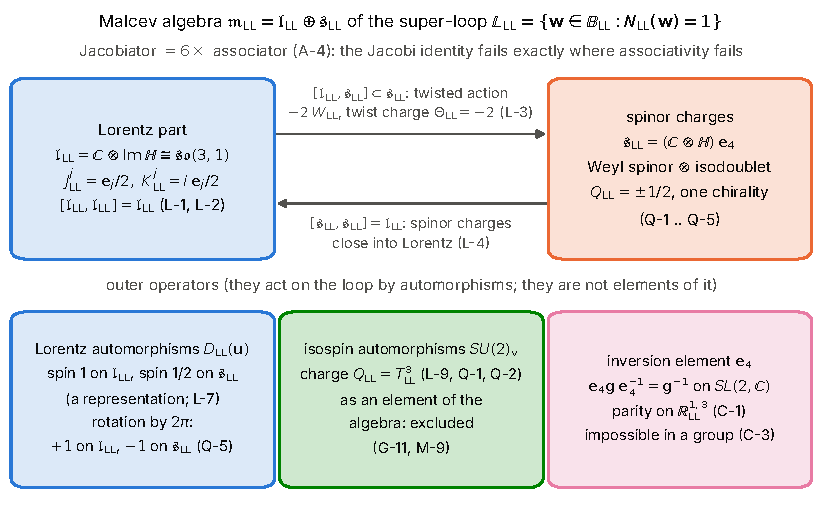
\includegraphics[width=\columnwidth]{../figures/fig_sl_superloop.pdf}
\caption{The Malcev algebra of the Lorentz super-loop: its Lorentz part $\mathfrak l_{\rm LL}$ and its
spinor charges $\mathfrak s_{\rm LL}$, their brackets, Eqs.~(\ref{eq:twist}) and~(\ref{eq:ss}), and the
outer operators of Sec.~\ref{sec:operators}, which act on the loop by automorphisms. The labels are
those of the machine checks.}
\label{fig:superloop}
\end{figure}

\subsection{The twist charge and the Jacobiators}

Define the \emph{twist charge} $\Theta_{\rm LL}$ as the linear map of $\mathfrak m_{\rm LL}$ that is $1$
on $\mathfrak l_{\rm LL}$ and $-2$ on $\mathfrak s_{\rm LL}$. With the Lorentz derivation $D_{\rm
LL}(\mathbf u)$ of Sec.~\ref{sec:operators}, which acts on $\mathfrak l_{\rm LL}$ by the commutator and on
$\mathfrak s_{\rm LL}$ by $W_{\rm LL}$, the inner action factors as $[\mathbf u,\cdot\,]=D_{\rm
LL}(\mathbf u)\circ\Theta_{\rm LL}$ (L-7). Suppose more generally that $\mathbf u$ acts on the spinor
charges by $\Theta_{\rm LL}W_{\rm LL}(\mathbf u)$ with any number $\Theta_{\rm LL}$. Then
\begin{align}
&\mathrm{Jac}_{\rm LL}(\mathbf u_1,\mathbf u_2,\mathbf b\,\mathbf e_4)\nonumber\\
&=\Big(\big(\Theta_{\rm LL}W_{\rm LL}([\mathbf u_1,\mathbf u_2])\nonumber\\
&\qquad-\Theta_{\rm LL}^2[W_{\rm LL}(\mathbf u_1),W_{\rm LL}(\mathbf u_2)]\big)\mathbf b\Big)\,\mathbf e_4\nonumber\\
&=(\Theta_{\rm LL}-\Theta_{\rm LL}^2)\,(W_{\rm LL}([\mathbf u_1,\mathbf u_2])\mathbf b)\,\mathbf e_4 ,
\label{eq:jacluu}
\end{align}
which vanishes for the Lie actions $\Theta_{\rm LL}=0$ (trivial) and $\Theta_{\rm LL}=1$ (the Weyl
representation) and equals $-6(W_{\rm LL}([\mathbf u_1,\mathbf u_2])\mathbf b)\mathbf e_4$ for the
super-loop, $\Theta_{\rm LL}=-2$ (L-5, exact on all 288 basis triples). The Jacobiators of three spinor
charges and of one Lorentz element with two spinor charges are non-zero as well, for example
$\mathrm{Jac}_{\rm LL}(\mathbf e_4,\mathbf e_5,\mathbf e_6)=-12\,\mathbf e_7$ (L-5).

\subsection{Theorem L: no Lie algebra does this}

\noindent\emph{Theorem L.} Let $\mathfrak l_{\rm LL}\oplus\mathfrak s_{\rm LL}$ carry a bracket that is
the Lorentz bracket on $\mathfrak l_{\rm LL}$, acts on $\mathfrak s_{\rm LL}$ covariantly, $[\mathbf
u,\mathbf b\mathbf e_4]=c^{\rm tw}_{\rm LL}(W_{\rm LL}(\mathbf u)\mathbf b)\mathbf e_4$, and has
$[\mathbf b\mathbf e_4,\mathbf b'\mathbf e_4]=c^{\rm sl}_{\rm LL}(\bar{\mathbf b}\mathbf b'-\bar{\mathbf
b}'\mathbf b)$, with complex numbers $c^{\rm tw}_{\rm LL}$, $c^{\rm sl}_{\rm LL}$. (Section~\ref{sec:classification}
shows that these are the most general Lorentz- and isospin-covariant brackets.) If the Jacobi identity
holds, then $c^{\rm sl}_{\rm LL}=0$: in a Lie algebra, bosonic spinor charges cannot close into the
Lorentz generators.

\noindent\emph{Proof.} By Eq.~(\ref{eq:jacluu}) with $\Theta_{\rm LL}=c^{\rm tw}_{\rm LL}$, the
Jacobi identity on $(\mathbf u_1,\mathbf u_2,\mathbf b\mathbf e_4)$ requires $c^{\rm tw}_{\rm LL}=0$ or
$1$. If $c^{\rm tw}_{\rm LL}=0$, the Jacobi identity on $(\mathbf u,\mathbf b\mathbf e_4,\mathbf b'\mathbf
e_4)$ reduces to $c^{\rm sl}_{\rm LL}[\bar{\mathbf b}\mathbf b'-\bar{\mathbf b}'\mathbf b,\mathbf u]=0$ for
every $\mathbf u$; the brackets span $\mathfrak l_{\rm LL}$ (L-4), whose center is zero, so $c^{\rm
sl}_{\rm LL}=0$. If $c^{\rm tw}_{\rm LL}=1$, the Jacobi identity on three spinor charges reads
$c^{\rm sl}_{\rm LL}\sum_{\rm cyc}(W_{\rm LL}(\bar{\mathbf b}\mathbf b'-\bar{\mathbf b}'\mathbf b)\mathbf
b'')\mathbf e_4=0$, the sum running over the three cyclic orders of $(\mathbf b,\mathbf b',\mathbf b'')$.
For $\mathbf b=\mathbf e_0$, $\mathbf b'=\mathbf e_1$, $\mathbf b''=\mathbf e_2$ the three brackets are
$2\mathbf e_1$, $-2\mathbf e_3$, $-2\mathbf e_2$, and the sum is $6c^{\rm sl}_{\rm LL}\mathbf e_7$; so $c^{\rm
sl}_{\rm LL}=0$. $\square$

Check L-6 verifies the last step on all basis triples, and the Gr\"obner-basis classification of
Sec.~\ref{sec:classification} confirms the theorem for all coefficients and extends it to the
Poincar\'e algebra and to an added isospin algebra (G-1, G-5, G-10). The same computation with
$c^{\rm tw}_{\rm LL}=-2$, $c^{\rm sl}_{\rm LL}=1$ gives $\mathrm{Jac}_{\rm LL}(\mathbf e_4,\mathbf
e_5,\mathbf e_6)=6c^{\rm tw}_{\rm LL}c^{\rm sl}_{\rm LL}\,\mathbf e_7=-12\,\mathbf e_7$, the value of
L-5: the super-loop violates the Jacobi identity, but it obeys the Malcev identity.
